%
\documentclass[12pt]{article}
\usepackage{amssymb}
\usepackage{amsmath}
\usepackage{graphicx}
\usepackage{epstopdf}
\usepackage{pdflscape}
\usepackage{tabularx}
\usepackage{longtable}
\usepackage{array}
\usepackage{dsfont}
\usepackage{float}
\usepackage{booktabs}
\usepackage{marvosym}
\usepackage{multirow}
\usepackage{pdflscape}
\usepackage[hyphenbreaks]{breakurl}
\usepackage[hyphens]{url}
\usepackage{setspace}
\usepackage{epigraph}
\usepackage{bm}
\usepackage{textcomp}
\usepackage{bbm}
\usepackage{verbatim}
\usepackage{subcaption}
\usepackage[format=hang,font={small,bf}]{caption}
\usepackage[shortlabels]{enumitem}
\usepackage{graphicx}
\usepackage{natbib,hyperref}
\setlength{\epigraphrule}{0pt}
\setlength\parindent{1cm}
\renewcommand{\baselinestretch}{1}
\renewcommand*{\arraystretch}{1.2}

\setcounter{MaxMatrixCols}{10}

\newcolumntype{L}[1]{>{\raggedright\let\newline\\\arraybackslash\hspace{0pt}}m{#1}}
\newcolumntype{C}[1]{>{\centering\let\newline\\\arraybackslash\hspace{0pt}}m{#1}}

\newcommand{\E}{\mathrm{E}}
\newcommand{\BLP}{\mathrm{BLP}}
\newcommand{\Var}{\mathrm{Var}}
\newcommand{\Cov}{\mathrm{Cov}}
\newcommand{\Corr}{\mathrm{Corr}}
\newcommand{\Prob}{\mathrm{P}}
\newcommand{\N}{\text{N}}

\topmargin=-1.5cm \textheight=23cm \oddsidemargin=-0.0cm
\evensidemargin=-0.0cm \textwidth=16.5cm
\newtheorem{ass}{Assumption}
\newtheorem{definit}{Definition}
\newtheorem{prop}{Proposition}
\newtheorem{thm}{Theorem}
\newtheorem{lem}{Lemma}
\newtheorem{conj}{Conjecture}
\newtheorem{cor}{Corollary}
\newtheorem{rem}{Remark}
\renewcommand{\thesubsection}{\arabic{section}.\arabic{subsection}}
\renewcommand{\thesubsubsection}{\arabic{section}.\arabic{subsection}.\arabic{subsubsection}}

\newcommand\independent{\protect\mathpalette{\protect\independenT}{\perp}}
\def\independenT#1#2{\mathrel{\rlap{$#1#2$}\mkern2mu{#1#2}}}

%Figure path
\def \figroot{stata/out/}
\def \tabroot{stata/out/}

\usepackage{epsfig,hyperref}

\hypersetup{
	pdftitle={ECMA31330 Final Project},    % title
	pdfauthor={Bronckers.Song.Zhang},     % author/Users/veronica/Documents/
	pdfnewwindow=true,      % links in new window
	colorlinks=true,       % false: boxed links; true: colored links
	linkcolor=blue,          % color of internal links
	citecolor=red,        % color of links to bibliography
	filecolor=black,      % color of file links
	urlcolor=blue           % color of external links
}

\allowdisplaybreaks


\begin{document}
\begin{titlepage}
    \begin{center}
        \vspace*{1cm}
        \LARGE
        \textbf{PAPER TITLE Blah Blah\\ Estimating Reaction to Welfare\\ Using Causal Forests\\}
        \vspace{0.5cm}
        \Large
        ECMA 31330 Final Project \\ 
        \vspace{0.8cm}
        \large
        Spring 2021
        \vfill
        \vspace{5cm}
        \textbf{Max Bronckers \\ Veronica Song \\ Dustin Zhang}
    \end{center}
\end{titlepage}


\section{Introduction} 
There has been an increasing adoption of Machine Learning (ML) methods in
economics for causal inference. While initially ML methods were avoided due to
an uncertainty in their consistency, normality, and efficiency, major developments in
methodology have allowed a stable large-sample confidence interval to be
constructed around treatment effect estimates conditional on multiple
covariates--leading to the broader adoption of these methods.~\cite{athey2019ML} \\

One such method is Bayesian Additive Regression Trees (BART), a non-parametric
method that models heterogeneous treatment effects flexibly by building on the
concept of ensembles of trees. Using a Markov Chain Monte Carlo (MCMC) algorithm
that derives effects from the posterior mean and interval instead of
pre-specified tree parameters, BART has a much smoother and adaptive structure
than traditional OLS or single tree models popular in economics, and is also
resilient to problems with overfitting.~\cite{greenkern2012} However, despite its
excellent predictive capacity, BART lacks an asymptotic explanation for its
estimates and is not guaranteed to converge in polynomial time
\cite{atheywager2019}, weakening its effectiveness as inference tool. Though
recent work by Ročková and Saha (2018) suggests modifications to BART that may
allow asypmtotic concentration of the posterior mean around the true mean, the
construction of an asymptotic theory of BART estimates is still an ongoing
effort.~\cite{rockova2018theory} An alternative method is the Causal Forest (CF),
proposed by Wager and Athey (2017). One of the advantages of CF is that their
estimates are asymptotically gaussian and unbiased, allowing proper confidence
intervals to be constructed around the treatment effect. The construction of
adequate confidence intervals is especially relevant in policy applications, as
consistent estimates can be produced for the treatment group.~\cite{atheywager2019} \\ 

In this paper, we evaluate Causal Forests as a method for heterogeneous
treatment effect estimation on both empirical and simulated datasets.
Specifically, we compare the CF method to BART in the estimation of heterogenous
treatment effects in a survey experiment on welfare opinions from the General
Social Survey as used by Green and Kern. Green and Kern use the GSS survey dataset with individual perception on public spending. To find the impact of the question phrasing on the responses, they use BART to estimate heterogeneous treatment effects by conditioning on a suite of socioeconomic backgrounds of the respondent. Given
the theoretical shortcomings of BART and the theoretical benefits of CFs, we
apply CFs to same problem and empirical dataset and compare it to the authors'
findings.

In section 2, we fit a CF model on the welfare data and compares our estimates against BART estimates of conditional average treatment effect (CATE) obtained by Green and Kern. Since empirical data offers no ground truth CATEs, we are confined to comparing the methods on interval length and RMSE. In section 3, we remedy this shortcoming with an evaluation of the CF method applied to DGPs that attempt to represent the empirical dataset. Using the ground truth ATE and CATEs of our DGPs, we assess the CF's performance under a variety of different DGP parameters and assess the conditions under which CFs perform well or poorly.
\\ 

\section{Causal Forest Estimates of CATE in Welfare Dataset} 

\subsection{Discussion of data and motivation for research} 
In our analysis below, we use a survey experiment from GSS which is also utilized by Green and Kern to investigate interactions between treatment and covariates that may lead to treatment effect heterogeneity. The experiment was conducted in the mid-1980s by GSS to study the negative sentiment Americans carry toward government programs labeled as "welfare". Due to associations with racial connotations and poorly managed welfare programs, respondents were found much more likely to endorse government spending for "the poor" than for public "welfare".~\cite{rasinski1989}\\

Using BART, Green and Kern illustrates the extent to which such reaction to the question wording as "welfare" varies based on the respondents' background characteristics such as years of education, race, or political alignment. BART has been a popular choice for heterogeneous treatment effect modeling, as its estimates require little parameter tuning, allow accurate detection of interactions between covariates, and are much smoother than those of single tree models. Each individual tree in the forest has only a small effect on the model, by assuming a prior distribution over the tree parameters.~\cite{Chipman2010} Such lack of any individual influential trees allow regular model fit of the BART set up. Then, a MCMC algorithm is used to sample tree parameters iteratively from the posterior distribution as the model is fit. Though this assumption of prior distribution and back-fitting algorithm allows BART to be relatively invariant across, in the presence of confounding variables and treatment effect heterogeneity, such regularization may severely bias the treatment effect estimates~\cite{CarvalhoHahnMurray}. Moreover, BART estimates still lack theoretical explanation on its asymptotic concentration, making the construction of adequate confidence intervals challenging. 

\subsection{Causal forests and model assumptions} 
For these reasons, we choose to investigate causal forests to estimate the the treatment effect of question wording on welfare program support. Just like BART, causal forests is fit to model non-linear relationships and interactions between covariates. One advantage that causal forests carry over BART is that under weak assumptions, the estimate are asymptotically standard normal distributed with Gaussian confidence intervals.~\cite{atheywager2019}. Put in context of economic policy, the presence of an asymptotic theory allows hypothesis testing regarding treatment results and thus aids policy decisions to be made. \\

Causal forests are a specific form of generalized random forests (GRF), which uses adaptive sample splitting criterion taking into account the MSE. To avoid overfitting and reduce bias in the estimates, we also ensure that the tree is 'honest' - the subsample with which we grow a tree is disparate from the subsample with which we drop down and obtain predictions. 
Additionally, we also note that although causal forests uncover heterogeneous treatment effects with valid confidence intervals for statistical inference, it does not necessarily address the affect of confounding due to the regularization on our trees. The terminal leaves of our tree are not homogenous across covariates for the sake of lowering variance and thus increasing precision, but with confounding within the leaves, we cannot guarantee that our treatment effect estimates will be unbiased. We thus use the Double/Debiased Machine Learning method (DML) for causal forests proposed by Chernozhukov et al. (2016) that uses orthogonalized treatment on covariates to estimate the treatment effect.~\cite{DML} We achieve this through the \textit{CausalForestDML} function. In our model, we use 80\% of the welfare data to build our tree and estimate treatment effects on the rest with a 5-fold CV for parameters of the model. \\ 

\subsection{Results of analysis and explanation}
We first investigate the average treatment effects (ATE) without conditioning on any covariates for possible effect heterogeneity. We obtain an ATE of 0.336, with a standard deviation of 0.049 and a 95\% confidence interval of (0.256, 0.416). Green and Kern (2012) identified seven variables to condition the treatment effects on: \textit{party identification, political views, age, education, negative attitude towards Blacks}, and \textit{survey year}. Figure 1 displays the CATE estimates obtained by the causal forest model conditional on each of the seven variables. The blue areas represent the 95\% confidence intervals of our estimates. \\

The top two graphs represents CATE as a function of party identification and self-identified political alignment from liberal to conservative. We see around 5 and 3 percentage points difference in the effect of question wording on support for welfare spending between strong Republicans-Democrats and Conservative-Liberals, respectively, controlling for all other covariates. Conservatives and strong Republicans are more likely to be affected by the framing of the survey question as for welfare. The treatment effect conditional on age, on the other hand, is greatest for those in their 30-40s, and diminishes past that age group. The negative bias toward Blacks has a less pronounced moderation on the treatment effect than the BART estimates.  We note that the trends in CATE estimates obtained via causal forest are generally similar to those obtained using BART for most of the covariate groups except education. There seems to be an increasing effect of question wording as the responded receives greater years of education, with the effect peaking at around 11-13 years (with college education). Whereas Green and Kern found no distinct moderation of treatment effects based on education, we find that there is around 5 percentage point difference in treatment effect estimates between those who received no education and those who received post-Graduate education. This indicates that more educated individuals respond more favorably to the question worded as 'assistance to the poor'. Lastly, we examine that change in CATE through time (survey year) and find that the treatment effect was strongest during years 1993-1996. Our results once again largely agree with the results obtained through BART, and illustrate that response to "welfare" is highly associated with the respondent's personal background characteristics. \\

We note that our CATE estimates from causal forest are on average lower than those of BART. The higher estimates of the BART estimates can be attributed to the regularization-induced confounding (RIC) identified by Hahn, Murray, and Carvalho (2019).\cite{CarvalhoHahnMurray} The treatment effect in BART is obtained by taking the conditional expectation of the outcome conditional on treatment and certain covariates: $E[Y|x,Z = 1] - E[Y|x,Z = 0]$, which in the presence of confounding in finite sample size, outcome may be dependent mostly on x rather than the treatment Z. RIC thus states that the obtained CATEs are heavily dependent on the regularization by the prior distribution in samples of defined sizes. \\

Figure 2 shows the overall presence of treatment effect heterogeneity in the sample. The histogram shows that treatment effect ranges from 10 percentage points to 52 percentage points, with the median estimated CATE of 34 percentage points. We note that compared to the BART median of 37 percentage points, we again obtain lower estimates on average. All estimates of CATE were positive, indicating that although the degrees of the response varies based on personal background covariates, all respondents react more favorably to a question framed for 'the poor' than for 'welfare'. \\

\textbf{Add Interpretation of results, Comparison to BART (Bias, RMSE, Coverage, Int length)?? TBD} 

\subsection{Suggestions for further analysis}
The causal forests approach also allows us to gauge covariate importance by calculating SHAP values, as indicated in figure 3.  We note that aside from the covariates estimated by Green and Kern, we find that variables as work status and racial backgrounds are also significant in the model. Although in this paper we limit the scope of our research to comparisons with the authors' estimates through BART, it may be meaningful in future research to estimate CATE conditional on those variables. 







\section{Testing Parameter Robustness of Causal Forest Estimates on Synthetic DGP} 

The analysis using the welfare data in the section above gives us an interesting real-life application of causal forest method; however, given the lack of ground truth in the empirical situation, we are unable to test the performance of our model in terms of metrics as bias and MSE. In this section, we explore multiple synthetic DGPs to estimate how causal forest performs under different data parameters. 

\subsection{Baseline DGP specification} 

We specify a DGP that resembles our empirical data using a simplified model of N individuals and 120 covariates. Each variable is drawn from a gaussian normal with mean and covariance obtained from the empirical data. We then take each randomly generated covariate and convert to its corresponding form. We assume that the outcome data is generated as: 
\[ Y = B \Gamma + T  \cdot \Theta(X) \tag{1} \label{eq:special}\]
where $\Gamma = X + \sum_{i = 0}^{I} X_i^\omega$ is the full list of covariates including their higher-order interactions with the \textit{i} most important features in the model. This parameter models the degree of linearity in the response surface: \textit{i} features are selected based on SHAP values obtained in the empirical analysis from section 1, and raised to the order of $\omega$ to model non-linear interactions and increased importance of these variables. In our baseline model, we sample N=5000 individuals with parameters $\omega = 3, i = 4$ for `med'-degree linearity. T, our treatment vector, models both binary and continuous treatment assignment; in the binary case, $ T \sim Binomial(n,p)$ where \textit{p} is the probability of receiving treatment (propensity score). We assume there is a 50\% probability of treatment in the baseline model. In the continuous case, we sample treatment from $T \sim Unif(0,1)$. We model heterogeneous or homogeneous treatment effects through $\Theta(X)$ as defined in equation (2). 
\[
\Theta(X) =  \begin{cases} 
	 \delta_H & {\{H = 0\}} \\ 
	 \delta_H \cdot \big( \sum_{j = 0}^{J} X_j + (\sum_{j = 0}^{J} X_j )^\omega ) & \{ H = 1 \} \\ 
\end{cases} \tag{2} \label{eq:special} \]
Variable \textit{H} indicates whether heterogenous treatment effects are present in the model ($H = 1$), and $\delta_H$ is the size of the effect. We take $\delta_0 = 10, \delta_1 = 2$ in the base model for each homogeneous and heterogeneous cases. $X_j$ parameters are again the \textit{j} most influential features in the empirical data as obtained by SHAP values. \\

\textbf{Also add about ATE stuff etc in baseline DGP} In the following analysis on parameter robustness of the model, we omit CATE estimation due to computational constraints. 

\subsection{DGP parameter modification and expectations of CF performance}

Based on the synthetic DGP above, we test the causal forest model for robustness by modifying the parameters. We then estimate the model \textit{K = 50} times for each parameter value in a range of different parameters. We consider the following dimensions for parameter tweaking: \textit{1) sample size, 2) non-linearity in covariates, 3) propensity score, 4) overlap, 5) degree of treatment effect heterogeneity,} and \textit{6) number of estimators}. 
\subsubsection{Sample size} 
In order to test the asymptotic theory of the causal forest estimates, we test the model performance on multiple sample sizes, $ N = \{1000, 5000, 10000\}$. We expect from standard statistics for both our bias and variance to decrease with increasing sample size, given our estimate converges to the true CATE value. Accordingly, interval length would also decrease.

\subsubsection{Linearity in response surface} 
We tweak the degree of linearity in our covariates to check if the causal forests model is able to handle higher degree relationships and complex interactions between variables. 4 degrees of linearity are explored, specified by \textit{i} in our definition of $\Gamma$ in equation (1) - which corresponds to \textit{full (i = 0), high (i=2), med (i=4), low (i=8)}. As causal forests are expected to be apt at detecting non-linear relationships than traditional treatment effect estimation methods as OLS, we would expect the model to be robust to the introduction of a non-linear response surface. 

\subsubsection{Propensity score} 
In this scenario, the data has an imbalanced treatment and control group sizes. Since treatment assignment is random with the propensity score $p = \pi(X)$ being constant across all individuals we do not expect this change to introduce any selection bias. However, as the ATE estimates are obtained by taking differences in means at the terminal node, the deviation in group sizes from a 50/50 split will likely harm the power of our model and increase the variance in our estimates. We estimate treatment probabilities of $p = \{0.1, 0.5, 0.9\}$ for extreme cases of imbalance. 

\subsubsection{Overlap}
We explore situations in which the propensity score \textit{p} satisfies or fails the overlap condition: $0 < p = \pi(X) < 1$. Given that in traditional statistical settings, overlap ensures there are observations on which we can estimate credible counterfactuals, we expect our causal forest estimate variances to increase without the condition. When overlap does not hold, we randomly sample half of the observations and force $T = 0$ to ensure that half the sample always has a 0\% probability of receiving treatment. 

\subsubsection{Degree of treatment effect heterogeneity} 
Causal forest optimizes sample-split by preferring leaves with heterogeneity in a key parameter and penalizing those with greater variance~\cite{athey2018grf}. The model is expected to show stable performance across the presence of complex heterogeneous effects. For this reason, we decide to alter the degree of treatment effect heterogeneity in the model, $\Theta(X)$, to check if the causal forest estimates are robust under such changes. We specify 4 different parameter values of $j = \{0,2,4,8\}$ for \textit{j} in equation (2). 

\subsubsection{Number of estimators} 
We vary the number of trees we fit in our causal forest estimator to see if our estimates are sensitive to tuning parameters. The baseline model had 1000 trees in each forest, and we expect with increasing number of trees we will be able to reduce overfitting and the importance of each tree in the estimate. Naturally, we believe the increase in this parameter will also show an increase in bias for CATE as our estimates are averaged out over multiple trees. However, this may not be as pronounced in the ATE estimate, which takes the average across the entire sample. We take the \textit{number of trees =} \{100, 500, 1000, 5000\} in each forest. 


\subsection{Results and discussion} 

Figure (4) and Table (1) illustrates the parameter resilience of causal forest ATE estimates for our specified DGP. 


\begin{table}
\caption{Model Performance with Parameter Variation}
\centering
\vspace{0.5cm}
\begin{subtable}{\textwidth}
\caption{Sample Size} 
\resizebox*{\textwidth}{!}{
\begin{tabular}{l|ccccccccc}
            \textbf{N} &\textbf{True ATE}&\textbf{Estimated ATE}&\textbf{Absolute Bias}&\textbf{Relative Bias}&\textbf{RMSE}&\textbf{Relative RMSE}&\textbf{Int. Length}&\textbf{Relative Int. Length}&\textbf{Coverage}\\
\toprule
\textbf{1000}         &    5439.607849	  &    5284.487310  &    173.520082	 &    0.031899	         &     202.689775  &    0.037262  & 1496.219129&    0.275060 &     1.0\\
\addlinespace
\textbf{5000}     &    5480.217592  &    5428.476930 &   53.144836	         &      0.009698  &       60.950723   &    0.011122  & 885.568983&    0.161594     &       1.0 \\
\addlinespace
\textbf{10000}         &    5464.342620  &    5437.754914 &    27.367210	 &    0.005008         &     30.277228 &    0.005541    & 706.760847 &    0.129341     &     1.0 \\
\bottomrule
\multicolumn{6}{p{\textwidth}}{\footnotesize Relative values calculated as percentage of estimated value compared to true population ATE}\\
\end{tabular}}
\end{subtable}

\begin{subtable}{\textwidth}
\vspace{0.5cm}
\caption{Linearity} 
\resizebox*{\textwidth}{!}{
\begin{tabular}{l|ccccccccc}
            \textbf{i} &\textbf{True ATE}&\textbf{Estimated ATE}&\textbf{Absolute Bias}&\textbf{Relative Bias}&\textbf{RMSE}&\textbf{Relative RMSE}&\textbf{Relative Int. Length}&\textbf{Int. Length}&\textbf{Coverage}\\
\toprule
\textbf{full}         &    5468.773915  &    5440.039188 &    36.353349 &    0.006647     &     45.801340	  &    0.008375  & 1.358807e+03 &    0.248466 &     1.0\\
\addlinespace
\textbf{high}     &    5453.578001	  &    5417.485903&   38.292994         &      0.007022	  &       47.719423   &    0.008750  & 1.289210e+03&    0.236397     &       1.0 \\
\addlinespace
\textbf{med}         &    5535.015621  &    5489.769929 &    45.867383 &    0.008287         &     56.011837 &    0.010120    & 8.908016e+02	&    0.160939     &     1.0 \\
\addlinespace
\textbf{low}         &    5455.065609  &    11248.379766 &   612400.414644  &    112.262704         &      813537.503514  &    149.134321    & 3.958072e+07 	&    7255.772887     &     1.0 \\
\bottomrule
\multicolumn{6}{p{\textwidth}}{\footnotesize Relative values calculated as percentage of estimated value compared to true population ATE}\\
\end{tabular}}
\end{subtable}

\begin{subtable}{\textwidth}
\vspace{0.5cm}
\caption{Propensity Score} 
\resizebox*{\textwidth}{!}{
\begin{tabular}{l|ccccccccc}
            \textbf{p} &\textbf{True ATE}&\textbf{Estimated ATE}&\textbf{Absolute Bias}&\textbf{Relative Bias}&\textbf{RMSE}&\textbf{Relative RMSE}&\textbf{Relative Int. Length}&\textbf{Int. Length}&\textbf{Coverage}\\
\toprule
\textbf{0.1}         &    5490.340503  &    5427.326138 &    132.827121 &    0.024193         &     179.524301  &    0.032698  & 1825.641746&    0.332519 &     1.0\\
\addlinespace
\textbf{0.5}     &    5481.328925  &    5449.166690&   36.238026         &      0.006611  &       45.833821   &    0.008362  & 881.562651&    0.160830     &       1.0 \\
\addlinespace
\textbf{0.9}         &    5469.355627  &    5387.042317 &    182.914155 &    0.033443         &     222.873837 &    0.040750    & 1803.281973&    0.329706     &     1.0 \\
\bottomrule
\multicolumn{6}{p{\textwidth}}{\footnotesize Relative values calculated as percentage of estimated value compared to true population ATE}\\
\end{tabular}}
\end{subtable}

\begin{subtable}{\textwidth}
\vspace{0.5cm}
\caption{Overlap} 
\resizebox*{\textwidth}{!}{
\begin{tabular}{l|ccccccccc}
            \textbf{overlap} &\textbf{True ATE}&\textbf{Estimated ATE}&\textbf{Absolute Bias}&\textbf{Relative Bias}&\textbf{RMSE}&\textbf{Relative RMSE}&\textbf{Relative Int. Length}&\textbf{Int. Length}&\textbf{Coverage}\\
\toprule
\textbf{True}         &    5453.466708  &    5403.129840 &    50.684381 &    0.009294         &     60.060401  &    0.011013  & 883.900621&    0.162081 &     1.0\\
\addlinespace
\textbf{False}     &    5456.466230  &    5404.707229 &102.429344 &      0.018772  &       128.709960   &    0.023589  & 1075.963858&    0.197191     &       1.0 \\
\bottomrule
\multicolumn{6}{p{\textwidth}}{\footnotesize Relative values calculated as percentage of estimated value compared to true population ATE}\\
\end{tabular}}
\end{subtable}

\begin{subtable}{\textwidth}
\vspace{0.5cm}
\caption{Degree of Heterogeneity} 
\resizebox*{\textwidth}{!}{
\begin{tabular}{l|ccccccccc}
            \textbf{j} &\textbf{True ATE}&\textbf{Estimated ATE}&\textbf{Absolute Bias}&\textbf{Relative Bias}&\textbf{RMSE}&\textbf{Relative RMSE}&\textbf{Relative Int. Length}&\textbf{Int. Length}&\textbf{Coverage}\\
\toprule
\textbf{0}         &    1.000000e+01  &    9.826431e+00 &    6.307467e-01 &    0.063075         &     8.345605e-01  &    0.083456  & 4.932942e+01&    4.932942 &     1.0\\
\addlinespace
\textbf{2}     &    	7.931915e+02  &    	7.874031e+02&   6.198745e+00         &      0.007815  &       7.912705e+00   &    0.009976  & 	1.647809e+02	&    0.207744     &       1.0 \\
\addlinespace
\textbf{4}         &    5.458236e+03  &    5.407529e+03 &    5.270965e+01 &    0.009657         &     6.209724e+01 &    0.011377    & 8.760214e+02	&    0.160495     &     1.0 \\
\addlinespace
\textbf{8}         &    1.262573e+10  &    1.256825e+10 &    1.283857e+08 &    0.010169         &     1.695761e+08 &    0.013431    & 3.384565e+09&    0.268069     &     1.0 \\
\bottomrule
\multicolumn{6}{p{\textwidth}}{\footnotesize Relative values calculated as percentage of estimated value compared to true population ATE}\\
\end{tabular}}
\end{subtable}

\begin{subtable}{\textwidth}
\vspace{0.5cm}
\caption{Number of Estimators} 
\resizebox*{\textwidth}{!}{
\begin{tabular}{l|ccccccccc}
            \textbf{Num\_Estimator} &\textbf{True ATE}&\textbf{Estimated ATE}&\textbf{Absolute Bias}&\textbf{Relative Bias}&\textbf{RMSE}&\textbf{Relative RMSE}&\textbf{Relative Int. Length}&\textbf{Int. Length}&\textbf{Coverage}\\
\toprule
\textbf{100}         &    5565.936961  &    5532.114094 &    33.822867 &    0.006077         &     33.822867  &    0.006077  & 1042.320012&    0.187268 &     1.0\\
\addlinespace
\textbf{500}     &    5523.942920	  &    5449.390716&   74.552204         &      0.013496	  &       74.552204   &    0.013496  & 830.519095&    0.150349     &       1.0 \\
\addlinespace
\textbf{1000}         &    5474.819893	  &    5450.791857	 &    24.028036 &    0.004389	         &     24.028036 &    0.004389    & 819.989987&    0.149775	     &     1.0 \\
\addlinespace
\textbf{5000}         &    5361.625270  &    5287.516977 &    74.108293 &    0.013822         &     74.108293 &    0.013822    & 840.772017 &    0.156813     &     1.0 \\
\bottomrule
\multicolumn{6}{p{\textwidth}}{\footnotesize Relative values calculated as percentage of estimated value compared to true population ATE}\\
\end{tabular}}
\end{subtable}
\end{table}



\section{Conclusion}
WRITESOME SHIT\\



\newpage
\bibliographystyle{abbrv}
\bibliography{Bibliography}

\begin{figure}[h]
\caption{CATE Estimates by Covariate}
\resizebox*{\textwidth}{!}{
	\centering
	\begin{subfigure} [h] {0.45\linewidth}
	\caption{\textbf{Party Identification}}
   	 	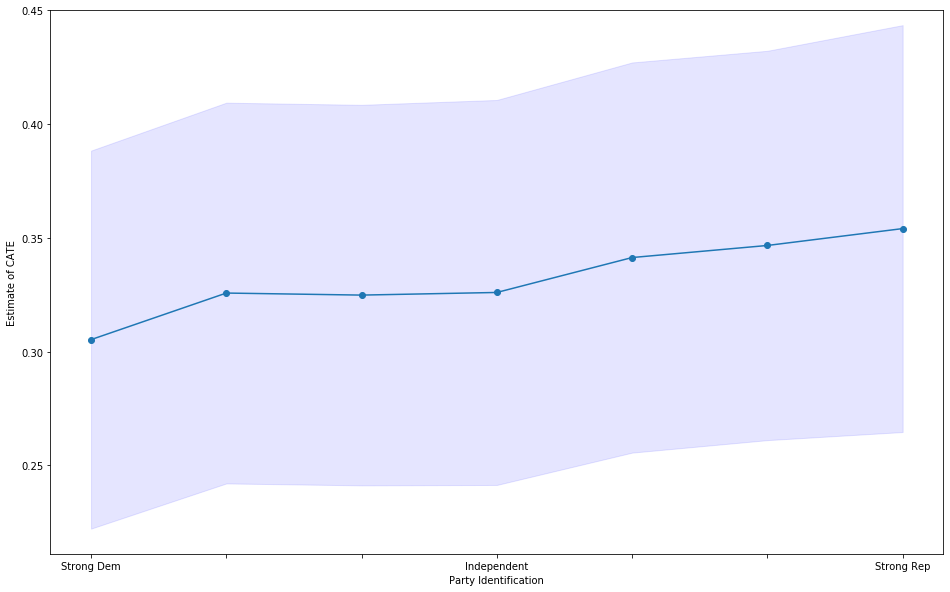
\includegraphics[width = \linewidth]{Graphs/s1_partyid.png}
	\end{subfigure}
	\begin{subfigure} [h] {0.45\linewidth}
		\caption{\textbf{Political Views}}
   	 	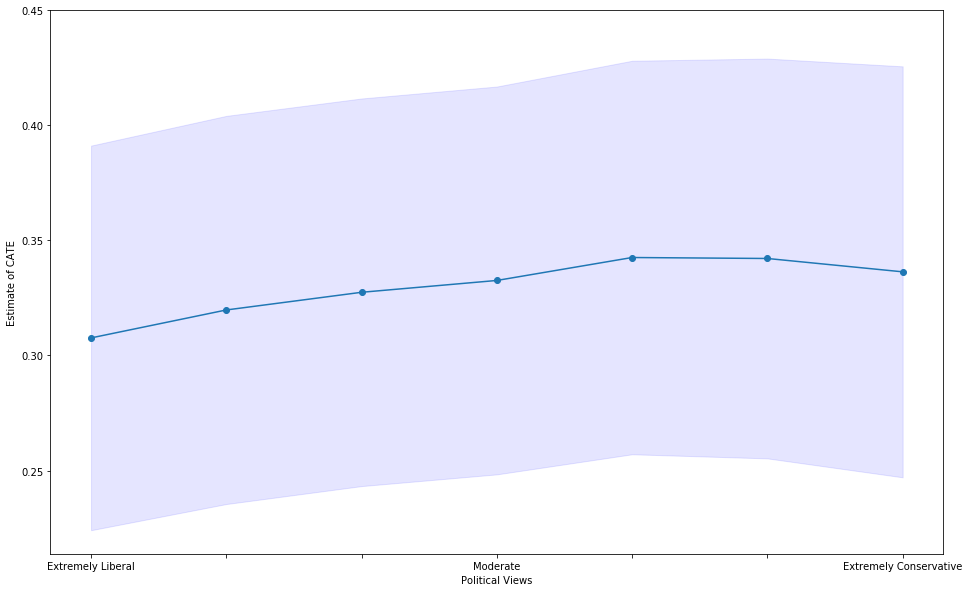
\includegraphics[width = \linewidth]{Graphs/s1_polyview.png}
	\end{subfigure}}
\resizebox*{\textwidth}{!}{
	\begin{subfigure} [h] {0.45\linewidth}
	\caption{\textbf{Age }}
   	 	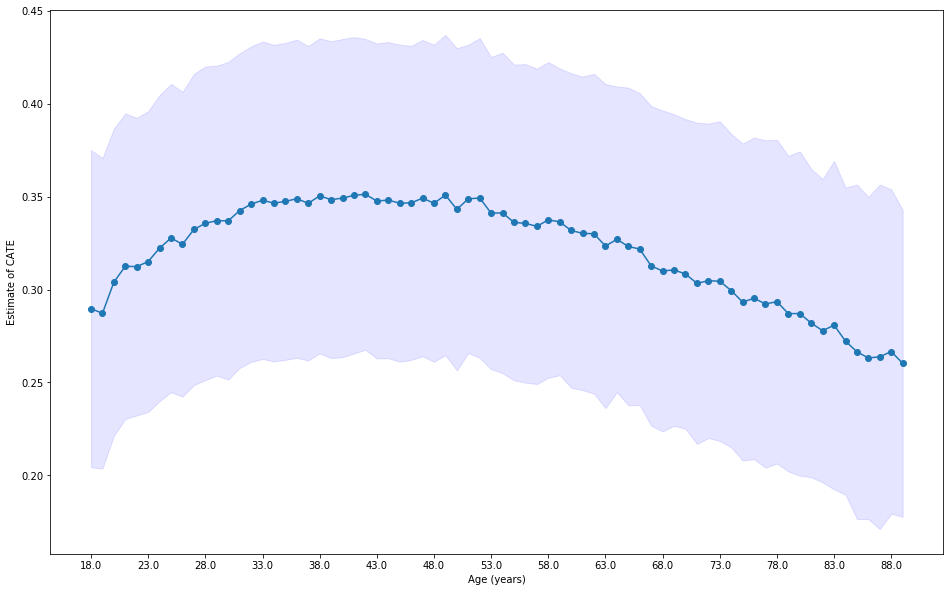
\includegraphics[width = \linewidth]{Graphs/s1_age.png}
	\end{subfigure}
	\begin{subfigure} [h] {0.45\linewidth}
		\caption{\textbf{Education Received}}
   	 	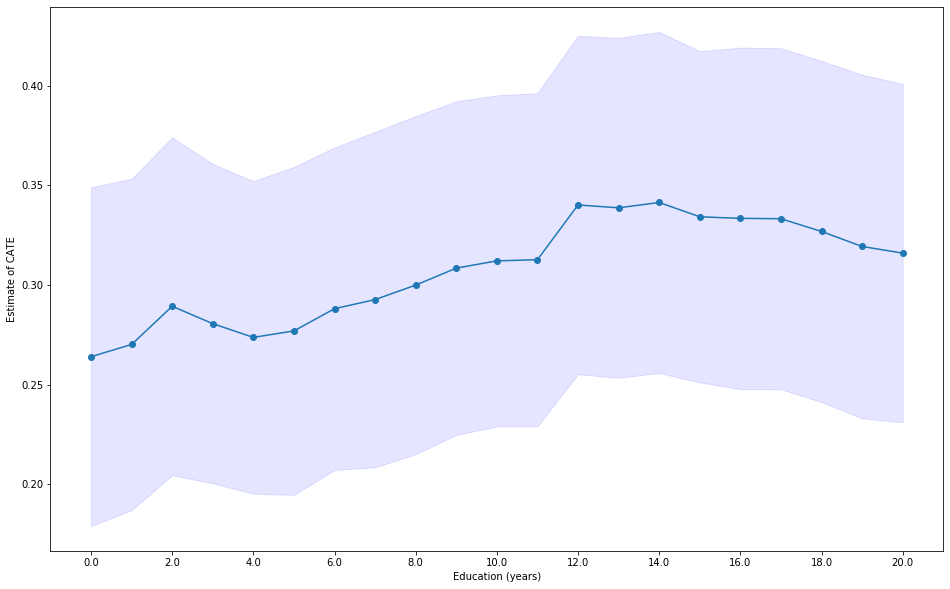
\includegraphics[width = \linewidth]{Graphs/s1_educ.png}
	\end{subfigure}}
\resizebox*{\textwidth}{!}{
	\begin{subfigure} [h] {0.45\linewidth}
	\caption{\textbf{Attitude Toward Blacks}}
   	 	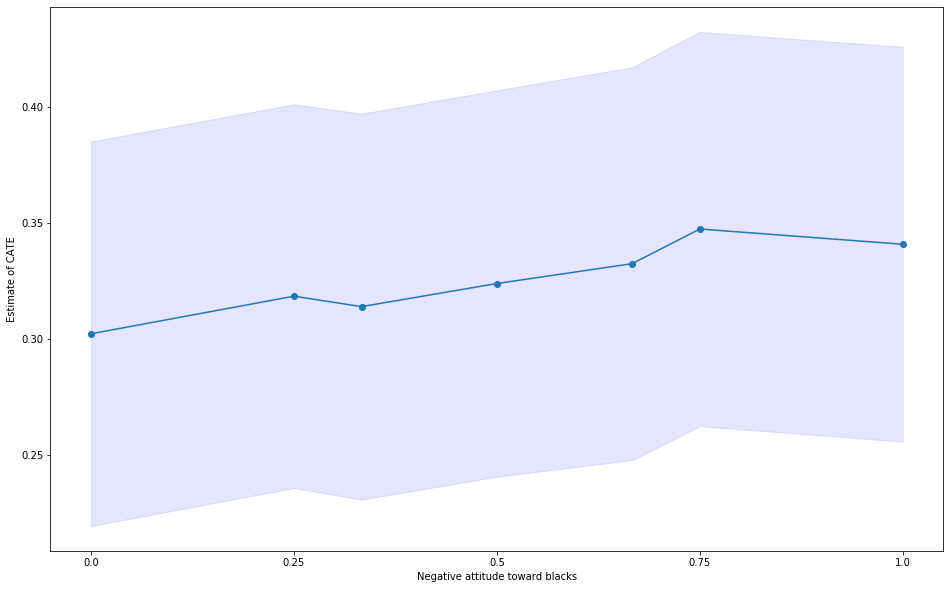
\includegraphics[width = \linewidth]{Graphs/s1_attblack.png}
	\end{subfigure}
	\begin{subfigure} [h] {0.45\linewidth}
		\caption{\textbf{Survey Year}}
   	 	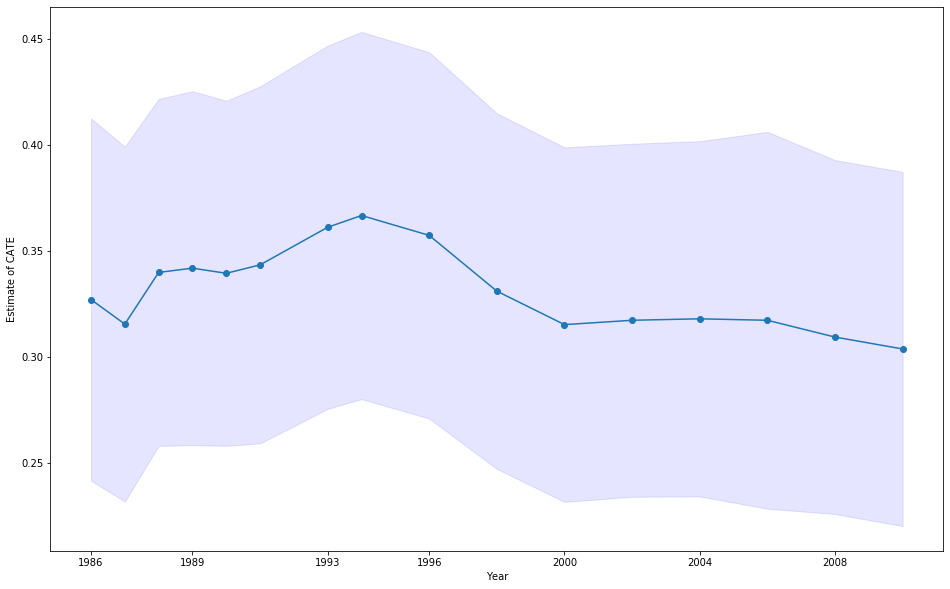
\includegraphics[width = \linewidth]{Graphs/s1_year.png}
	\end{subfigure}}
\end{figure} 

\begin{figure}[h]
\caption{Histogram of CATE Estimates}
	\centering
   	 	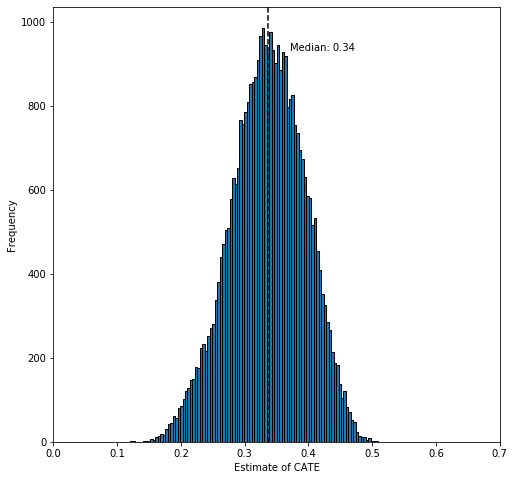
\includegraphics[width = 0.6\linewidth]{Graphs/s1_catefreq.png}
\end{figure} 

\begin{figure}[h]
\caption{Summary of SHAP Values of Covariate Importance}
	\centering
   	 	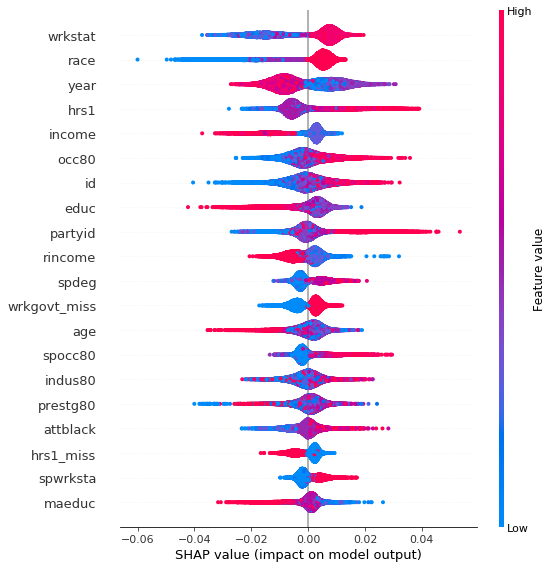
\includegraphics[width = 0.6\linewidth]{Graphs/s1_shap.png}
\end{figure} 

\begin{figure}[h]
\caption{Model Performance by Parameter Variation }
	\centering
	\begin{subfigure} [h] {\linewidth}
		\caption{\textbf{Sample Size}}
   	 	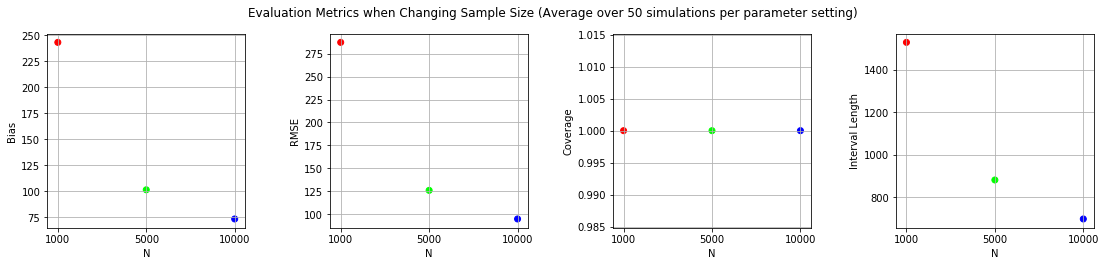
\includegraphics[width = \linewidth]{Graphs/s2_nsiz.png}
	\end{subfigure}
	\begin{subfigure} [h] {\linewidth}
\vspace{0.5cm}
		\caption{\textbf{Linearity}}
   	 	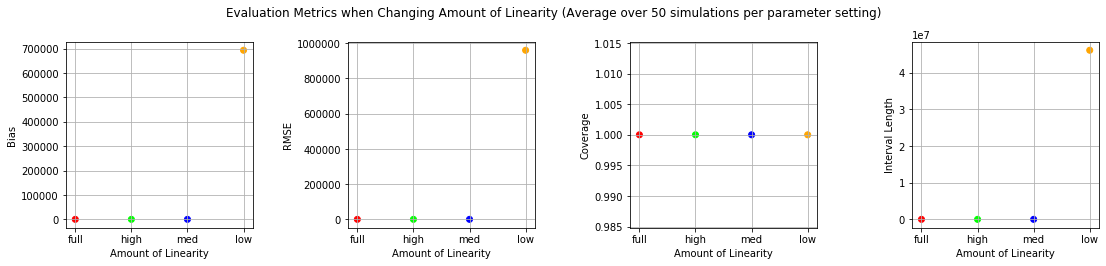
\includegraphics[width = \linewidth]{Graphs/s2_linear.png}
	\end{subfigure}
	\begin{subfigure} [h] {\linewidth}
\vspace{0.5cm}
		\caption{\textbf{Propensity Score}}
   	 	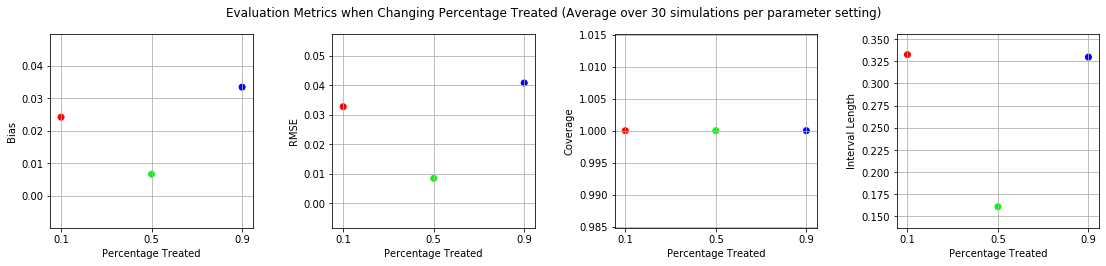
\includegraphics[width = \linewidth]{Graphs/s2_propen.png}
	\end{subfigure}
	\begin{subfigure} [h] {\linewidth}
\vspace{0.5cm}
		\caption{\textbf{Overlap}}
   	 	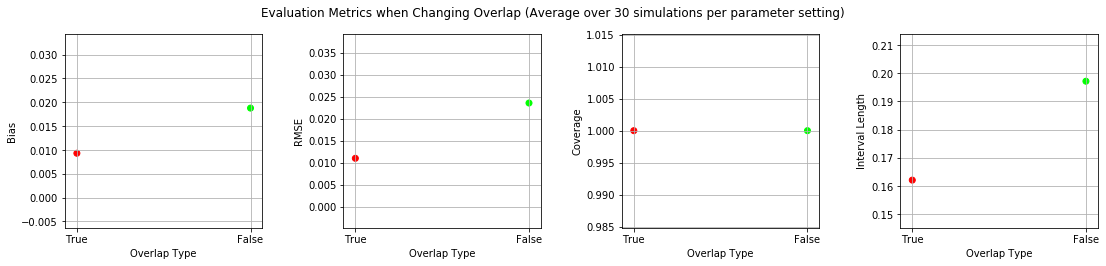
\includegraphics[width = \linewidth]{Graphs/s2_overlap.png}
	\end{subfigure}
\end{figure} 

\begin{figure}
\ContinuedFloat
	\begin{subfigure} [t] {\linewidth}
		\caption{\textbf{Degree of Heterogeneity}}
   	 	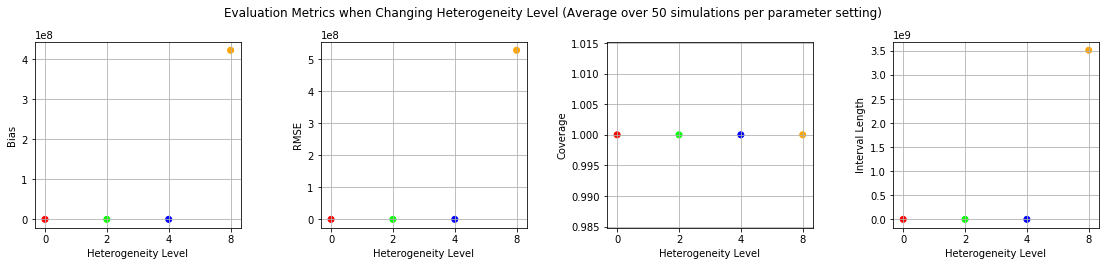
\includegraphics[width = \linewidth]{Graphs/s2_hetero.png}
	\end{subfigure}
	\begin{subfigure} [t] {\linewidth}
\vspace{0.5cm}
		\caption{\textbf{Number of Estimators}}
   	 	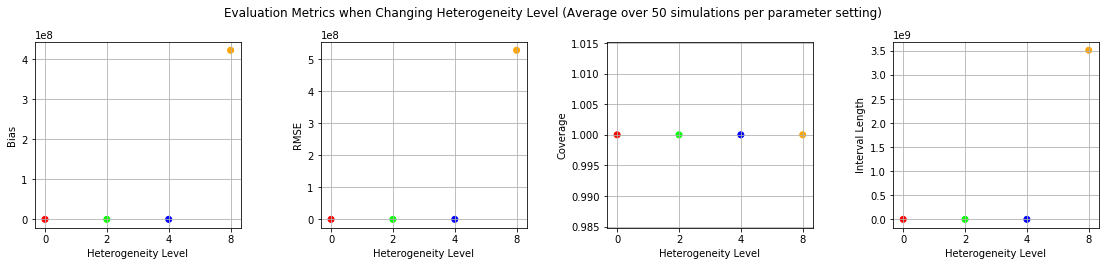
\includegraphics[width = \linewidth]{Graphs/s2_nestimator.png}
	\end{subfigure}
\end{figure} 




\end{document}



















